\chapter{Commande des robots manipulateurs I: quasi-statique}
\label{sec:staticcontrol}


Les objectifs en termes de mouvement désiré d'un robot sont généralement plus naturellement spécifiés en termes de variables dans l'espace de la tâche d'un robot, alors que à bas niveau les consignes des actionneurs sont reliés à des variables dans l'espace des joints. Ce chapitre présente des méthodes de commande qui permettent de calculer les consignes pour les actionneurs basé sur des objectifs directement spécifié dans l'espace de la tâche, malgré la relation géométrique hautement non-linéaire. Les méthodes ici présenté utilisent grandement les notions de cinématique différentiel et de statique présentés dans les sections \ref{sec:differentialkinematicmanipulators} et XXX.

Les méthodes présentés dans ce chapitre négligent les effets dynamiques (inerties, frottement, etc.) et considèrent juste un comportement simplifié des robots: la relation statique non-linéaire entre le mouvement/force des actionneurs et le mouvement/force à l'effecteur. Ces méthodes sont généralement performante lorsque les mouvements du robot sont relativement lents, c'est pourquoi ils sont ici regroupé sous la caractéristique "quasi-statique". Ensuite, selon la nature des actionneurs des systèmes robotiques, différentes variantes peuvent être utilisée:

\paragraph{Actionneurs commandés en vitesse:} Pour les méthodes de commande du mouvement de l'effecteur présentées aux sections \ref{sec:speedcontrol}, \ref{sec:positioncontrol} et \ref{sec:admcontrol}, il est considéré que le robot a des asservissements bas-niveau en vitesse à chacun des joints. Ces méthodes calculent les consignes en vitesse à envoyer aux joints pour contrôler le mouvement de l'effecteur. Ces méthodes fonctionnent bien dans des situations ou le suivi de consigne en vitesse des joints est très performant, c'est généralement le cas des manipulateurs industriels qui ont de très grand ratios de réduction. 

\paragraph{Actionneurs commandés en force:} Pour les méthodes de commande présentées aux section \ref{sec:forcecontrol} et \ref{sec:impcontrol}, on considère seulement la relation géométrique entre les forces des actionneurs et ceux à l'effecteur. Les deux méthodes calculent des forces à appliquer au niveau des actionneurs/joint, pour contrôler la force au niveau de l'effecteur. Ces méthodes fonctionnent donc bien pour des systèmes robotisées à basse impédance (peu d'inertie, peu d'effets dissipatifs, transmission réversibles, etc.), comme les systèmes haptiques où les forces des actionneurs sont pratiquement proportionnelles au courant dans les moteurs du à des très petits ratio de transmissions.



%%%%%%%%%%%%%%%%%%%%%%%%%%%%%%%%%%%%%%%%%%%%%%%%%%%%%%
\newpage
\section{Commande en vitesse de l'effecteur}
\label{sec:speedcontrol}
%%%%%%%%%%%%%%%%%%%%%%%%%%%%%%%%%%%%%%%%%%%%%%%%%%%%%%

Si un robot a des actionneurs contrôlés en vitesse à bas niveau, contrôler la vitesse de son effecteur se résume à mettre en oeuvre la relation de cinématique différentielle inverse (voir section \ref{sec:differentialkinematicmanipulators}).  Comme illustré par un schéma bloc à la Figure \ref{fig:robotspeedcontrol}, les consignes en vitesse pour les actionneurs sont déterminés en multipliant le vecteur-colonne de vitesses désirés dans l'espace des tâches, par l'inverse du Jacobien qui relie l'espace des joints à l'espace des tâches du systèmes. Le Jacobien est généralement dépendent de la position des joints du robot ce qui nécessite une boucle de rétroaction basé sur les capteurs de position des actionneurs pour effectuer le calcul de $J$ en continu basé sur la position actuel. Finalement, comme mis en évidence à la Figure \ref{fig:robotspeedcontrol}, cette méthode s'intègre comme une boucle haut-niveau pour coordonner les différents joints d'un système ou chacun des actionneurs est asservis en vitesse, souvent des boucles bas-niveaux implémentées directement dans l'électronique de contrôle des moteurs. 
%%%%%%%%%%%%%%%%%%%%%%%%%%%%%%%%
\begin{figure}[H]
	\centering
		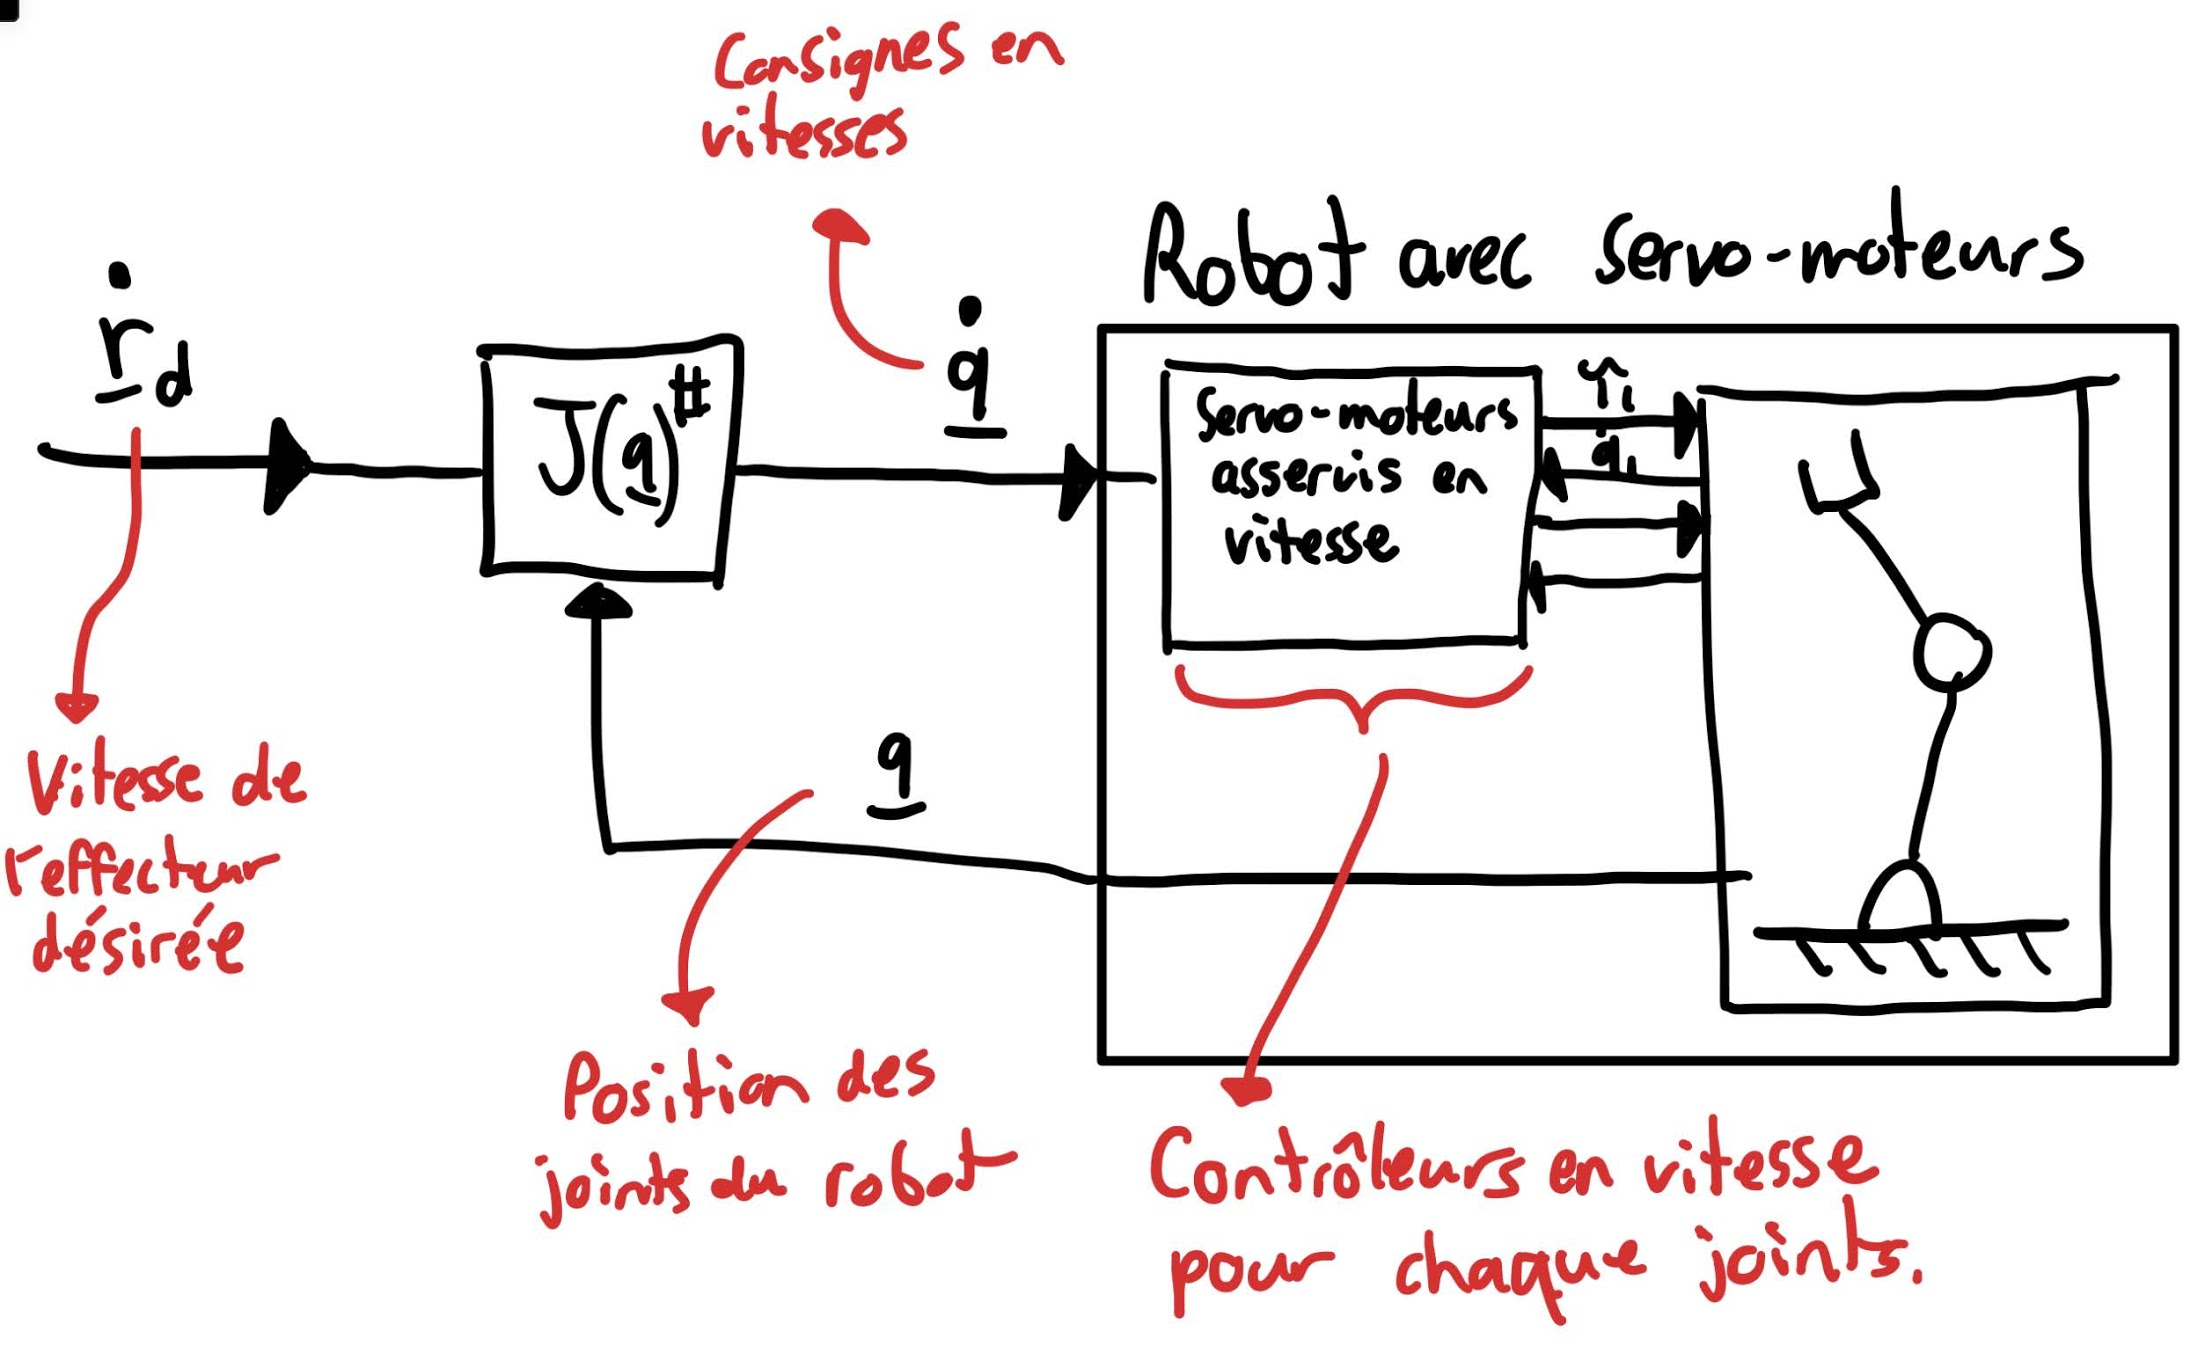
\includegraphics[width=0.7\textwidth]{fig/robotspeedcontrol.jpg}
	\caption{Commande de la vitesse de l'effecteur d'un robot : schéma bloc}
	\label{fig:robotspeedcontrol}
\end{figure}
%%%%%%%%%%%%%%%%%%%%%%%%%%%%%%%%

Si le nombre de joints $n$ est égale au nombre de DDL de l'espace de la tâche $m$, alors la matrice Jacobien est carrée et peut être inversée (sauf sur les singularités). Si le nombre de joint $n$ est supérieur au nombre de DDL de l'espace de la tâche $m$, alors on peut utiliser une matrice pseudo-inverse droite $J^{\#} = J^T (J J^T)^{-1}$ (voir section \label{sec:pseudoinverse}). La loi de commande en équation peut donc être exprimée comme:
%%%%%%%%%%%%%%%%%%
\begin{align}
\dot{\col{q}} = \left\{ \begin{array}{c}
 J(\col{q})^{-1} \dot{\col{r}_d}   \quad\quad \text{if $n=m$}
 \\ \\
 J(\col{q})^{\#} \, \dot{\col{r}_d}   \quad\quad \text{if $n>m$}
\end{array}
\right.
\end{align}
%%%%%%%%%%%%%%%%%

En substituant la loi de commande dans la relation de cinématique différentielle, on confirme que la vitesse de l'effecteur sera exactement la vitesse désirée:
%%%%%%%%%%%%%%%%%%
\begin{align}
\dot{\col{r}} &= J(\col{q}) \, \dot{\col{q}} \\
\dot{\col{r}} &= J(\col{q}) \, J(\col{q})^{\#} \, \dot{\col{r}_d} \\
\dot{\col{r}} &= J J^T (J J^T)^{-1} \, \dot{\col{r}_d} \\
\dot{\col{r}} &=  \dot{\col{r}_d} 
\end{align}
%%%%%%%%%%%%%%%%%
sous les hypothèses que: 1) le Jacobien utilisé par le contrôleur est exacte, 2) le Jacobien est inversible (i.e. le robot n'est pas sur une singularité) et 3) la vitesse des joints est parfaitement asservis par les boucles bas-niveaux. 




%%%%%%%%%%%%%%%%%%%%%%%%%%%%%%%%%%%%%%%%%%%%%%%%%%%%%%
\newpage
\section{Commande en position de l'effecteur}
\label{sec:positioncontrol}
%%%%%%%%%%%%%%%%%%%%%%%%%%%%%%%%%%%%%%%%%%%%%%%%%%%%%%

Pour commander la position de l'effecteur d'un robot, tenter de trouver une solution directement au problème de cinématique inverse (voir section \ref{sec:invkin} n'est généralement pas la méthode la plus appropriée car la cinématique directe des manipulateurs est hautement non-linéaire. La méthode ici présentée utilise plutôt la méthode de commande en vitesse de l'effecteur (section \ref{sec:speedcontrol}) pour indirectement résoudre la cinématique inverse du robot. L'idée ce résume à: si on peut contrôler la vitesse de l'effecteur de façon arbitraire, il suffit de diriger le vecteur vitesse de l'effecteur vers la position cible. La méthode est illustrée graphiquement à la Figure \ref{fig:robotspeedcontrolgeo}: 1) Un vecteur d'erreur $\col{r}_e$ est calculé en comparant la position désirée $\col{r}_d$ à la position actuelle $\col{r}$. 2) Le vecteur d'erreur $\col{r}_e$ est multiplié par un paramètre scalaire $\lambda$ pour déterminer la vitesse cible instantanée pour l'effecteur notée $\dot{\col{r}}_r$, qui point en direction de la cible. 3) L'inverse du Jacobien est utilisé pour convertir la vitesse instantanée désirée de l'effecteur en consigne de vitesse pour les joints. 
%%%%%%%%%%%%%%%%%%%%%%%%%%%%%%%%
\begin{figure}[H]
	\centering
		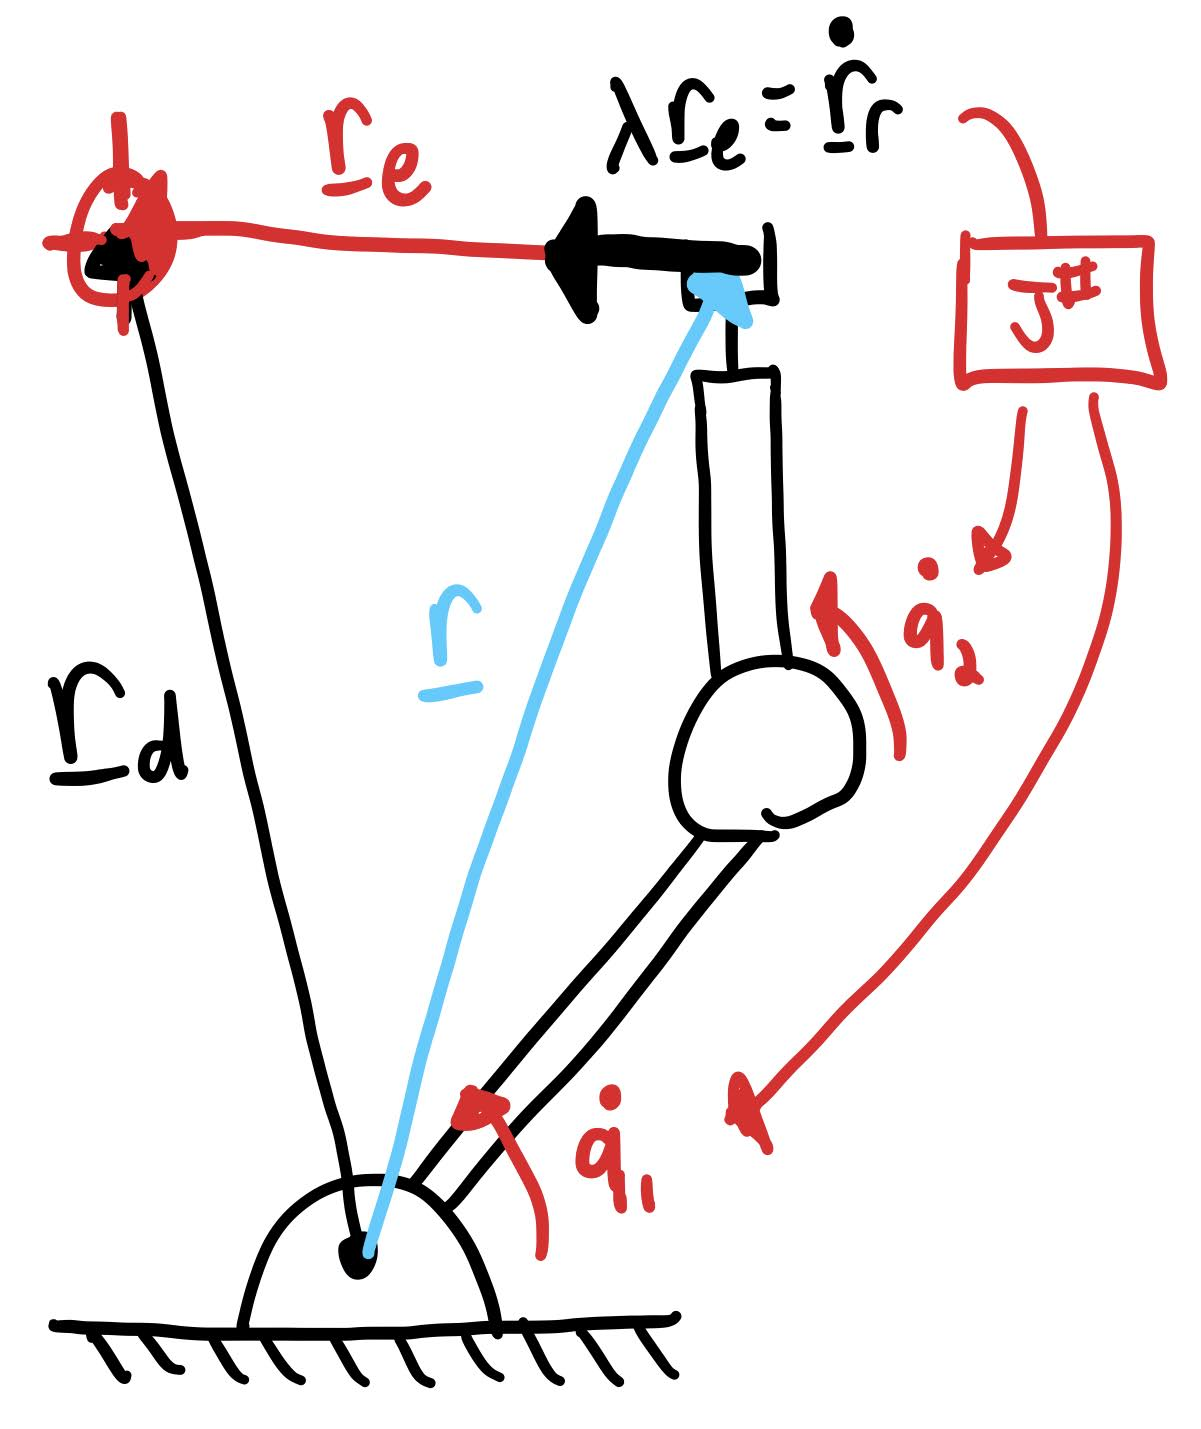
\includegraphics[width=0.4\textwidth]{fig/robotspeedcontrolgeo.jpg}
	\caption{Commande de la trajectoire de l'effecteur d'un robot : interprétation géométrique}
	\label{fig:robotspeedcontrolgeo}
\end{figure}
%%%%%%%%%%%%%%%%%%%%%%%%%%%%%%%%
Formellement, la loi de commande est exprimée par l'expression mathématique:
%%%%%%%%%%%%%%%%%%
\begin{align}
\dot{\col{q}} = \left\{ \begin{array}{c}
 J(\col{q})^{-1} \lambda 
 \underbrace{ \left( \col{r}_d  - \underbrace{f(\col{q})}_{\col{r}}  \right) }_{\col{r}_e} 
 \quad\quad \text{if $n=m$}
 \\ \\
 J(\col{q})^{\#} \, \lambda  \underbrace{ \left( \col{r}_d  - \underbrace{f(\col{q})}_{\col{r}}  \right) }_{\col{r}_e}    \quad\quad \text{if $n>m$}
\end{array}
\right.
\end{align}
%%%%%%%%%%%%%%%%%
ou $\lambda$ est un paramètre scalaire de gain du contrôleur, $J$ est le Jacobien, la matrice $n \times m$, qui relie l'espace des joints à l'espace de la tâche du manipulateur, et $f(\col{q})$ la fonction de cinématique directe du manipulateur. La Figure \ref{fig:robotspeedcontrolpos} illustre cette méthode de commande sous la forme d'un schéma bloc. 
%%%%%%%%%%%%%%%%%%%%%%%%%%%%%%%%
\begin{figure}[H]
	\centering
		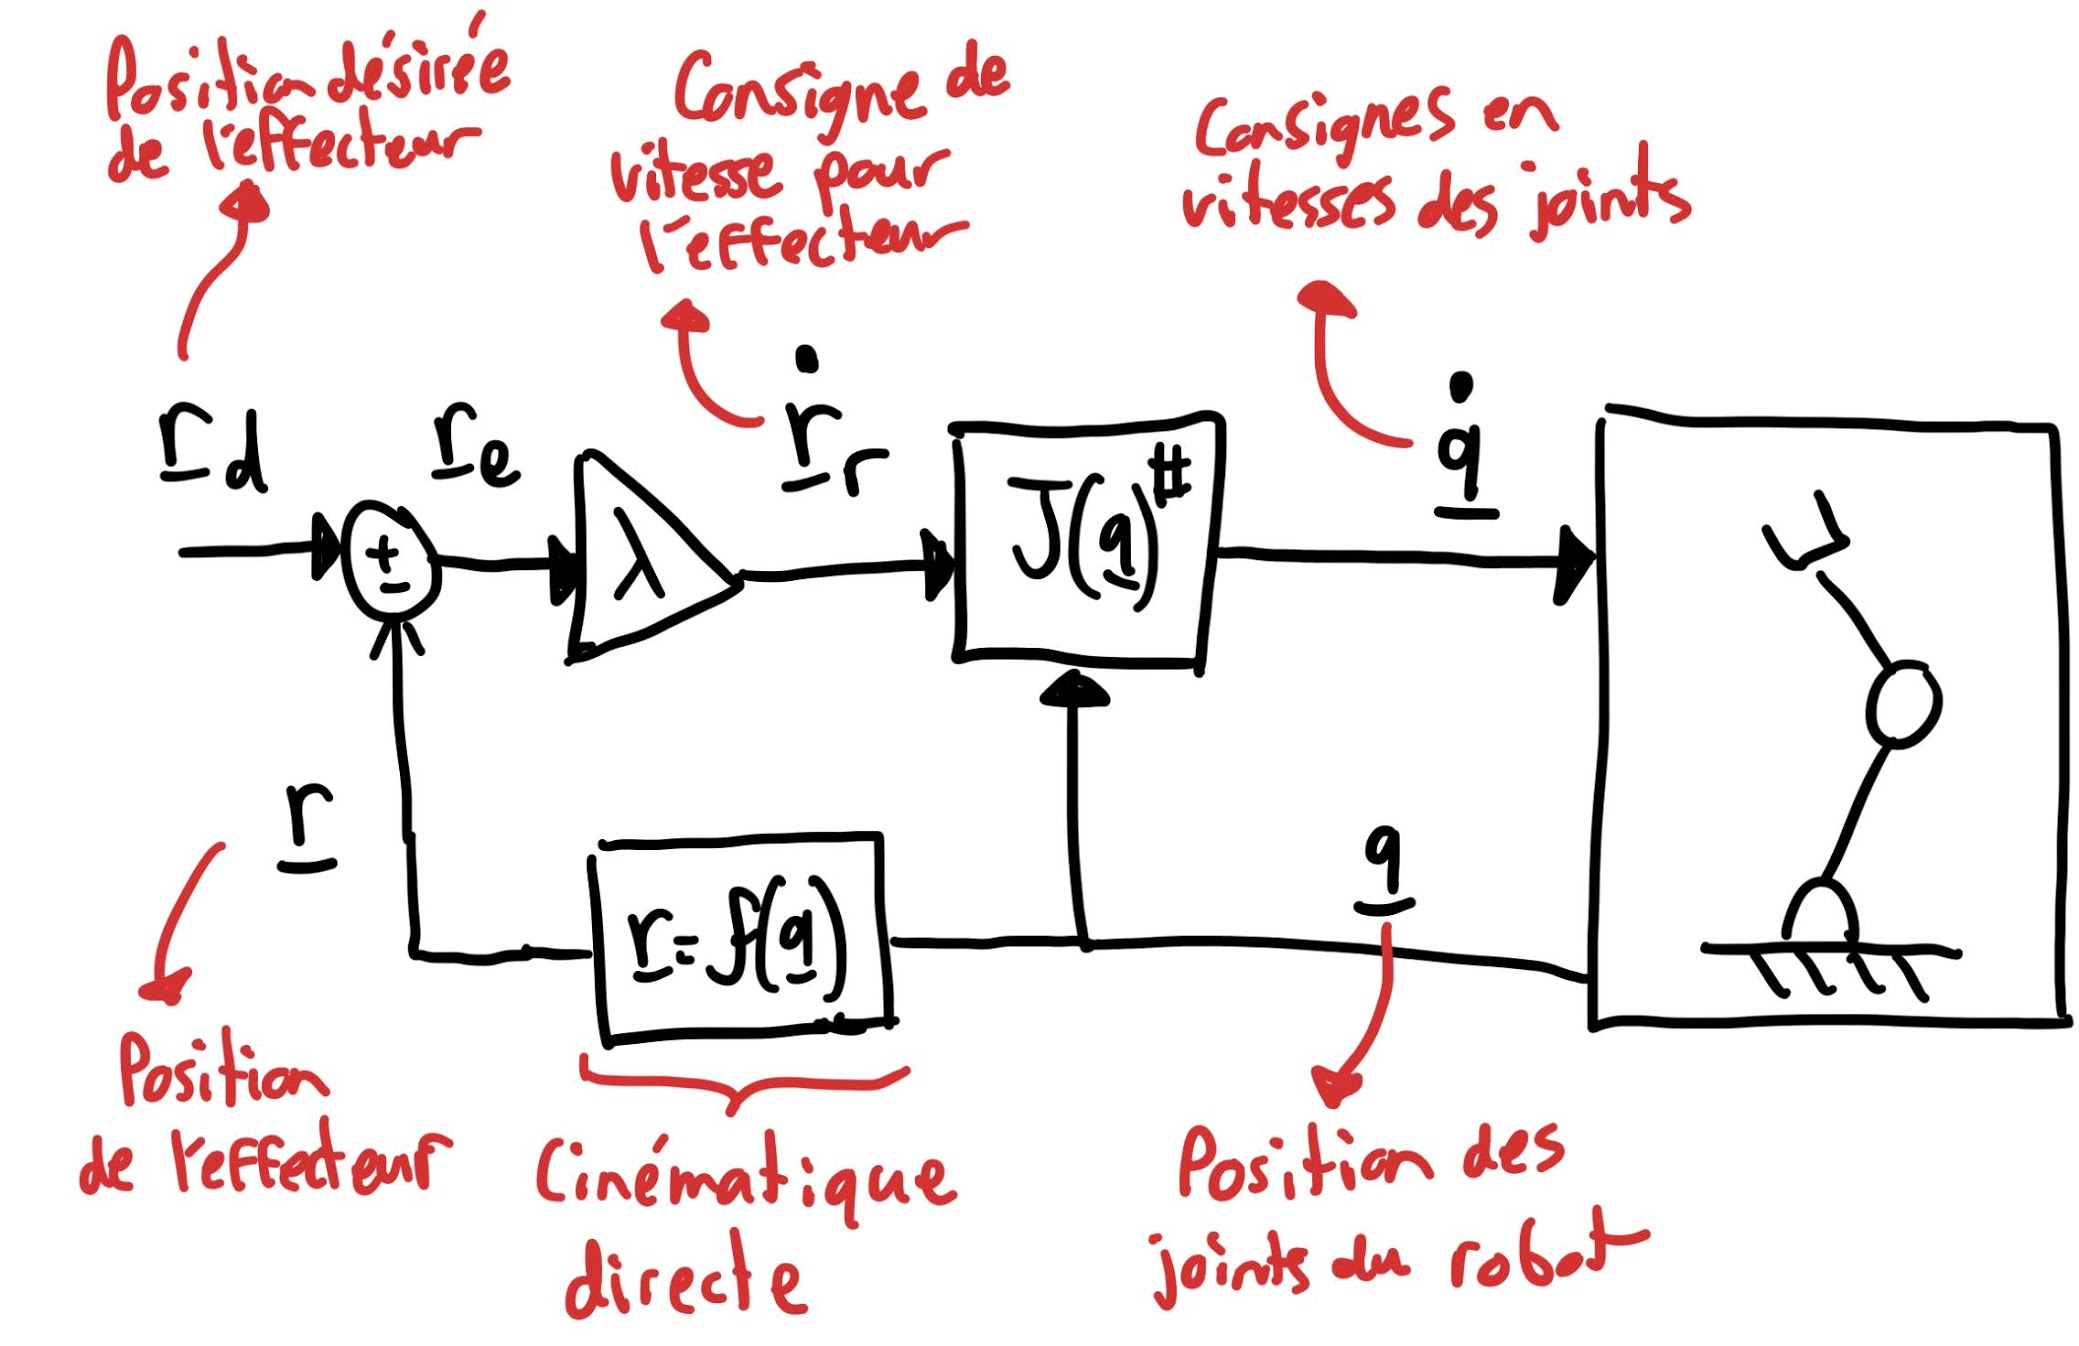
\includegraphics[width=0.7\textwidth]{fig/robotspeedcontrolpos.jpg}
	\caption{Commande de la position de l'effecteur d'un robot : schéma bloc}
	\label{fig:robotspeedcontrolpos}
\end{figure}
%%%%%%%%%%%%%%%%%%%%%%%%%%%%%%%%










%%%%%%%%%%%%%%%%%%%%%%%%%%%%%%%%%%%%%%%%%%%%%%%%%%%%%%%%%%%%%%%%
\subsection{Suivi de trajectoire}
\label{sec:trajcontrol}

Lorsque le robot doit suivre une position cible de l'effecteur qui varie dans le temps, il est préférable de calculer la dérivée temporelle de la trajectoire et d'utiliser cette information directement dans la loi de commande comme indiqué dans l'équation suivante:
%%%%%%%%%%%%%%%%%%
\begin{align}
\dot{\col{q}} = \left\{ \begin{array}{c}
 J(\col{q})^{-1} \left[ \dot{\col{r}_d} + \lambda \left( \col{r}_d  - \underbrace{f(\col{q})}_{\col{r}} \right) \right] \quad\quad \text{if $n=m$}
 \\ \\
 J(\col{q})^{\#} \, \left[ \dot{\col{r}_d} + \lambda \left( \col{r}_d  - \underbrace{f(\col{q})}_{\col{r}} \right) \right]   \quad\quad \text{if $n>m$}
\end{array}
\right.
\end{align}
%%%%%%%%%%%%%%%%%
En terme de schéma bloc, la vitesse de la trajectoire doit être utilisée avec un feedfoward dans la loi de commande comme illustré à la Figure \ref{fig:robotspeedcontroltraj}, pour garantir la convergence sur la trajectoire.
%%%%%%%%%%%%%%%%%%%%%%%%%%%%%%%%
\begin{figure}[H]
	\centering
		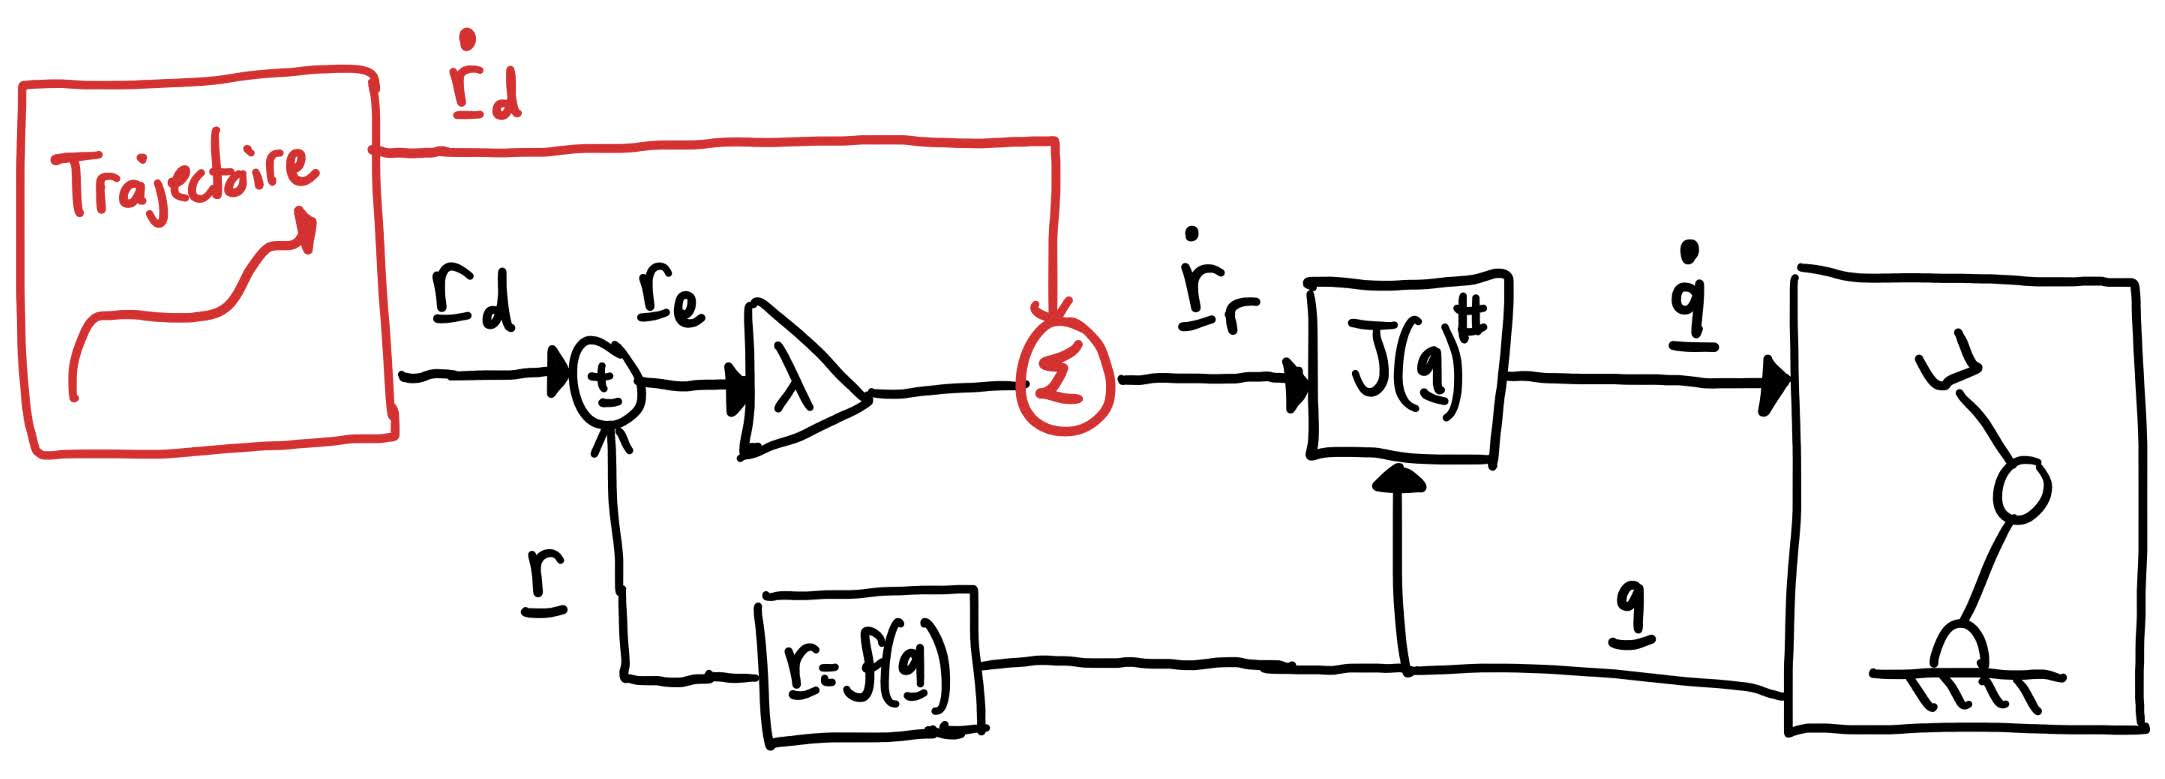
\includegraphics[width=0.95\textwidth]{fig/robotspeedcontroltraj.jpg}
	\caption{Commande de la trajectoire de l'effecteur d'un robot : schéma bloc}
	\label{fig:robotspeedcontroltraj}
\end{figure}
%%%%%%%%%%%%%%%%%%%%%%%%%%%%%%%%


\subsection{Convergence}

Les méthodes de commande en position de l'effecteur converge sous certaines conditions. L'objectif peut être mathématiquement exprimé comme:
%%%%%%%%%%%%%%%%%%
\begin{align}
\lim_{t \rightarrow \infty } \col{r}_e(t) = 0 
\end{align}
%%%%%%%%%%%%%%%%%
c'est-à-dire l'erreur (sur la position de l'effecteur) doit converger vers zéro. L'erreur est une fonction de la trajectoire et de la positon réelle du robot:
%%%%%%%%%%%%%%%%%%
\begin{align}
\col{r}_e = \col{r}_d - \col{r}
\end{align}
%%%%%%%%%%%%%%%%%
Si on dérive cette équation dans le temps, on obtient une relation différentielle. On peut alors substituer le modèle de cinématique différentiel et les lois de commandes pour obtenir:
%%%%%%%%%%%%%%%%%%
\begin{align}
\dot{\col{r}}_e 
&= \dot{\col{r}}_d - \dot{\col{r}} \\
&= \dot{\col{r}}_d - J(\col{q}) \dot{\col{q}} \\
&= \dot{\col{r}}_d - \underbrace{J(\col{q}) J(\col{q})^{\#} }_{1} \dot{\col{r}}_r \\
&= \dot{\col{r}}_d - \underbrace{J(\col{q}) J(\col{q})^{\#} }_{1}  \left( \dot{\col{r}}_d - \lambda \, \col{r}_e \right) \\
&= - \lambda \, \col{r}_e  
\end{align}
%%%%%%%%%%%%%%%%
La dynamique de l'erreur est donc stable et converge exponentiellement vers zéro si $\lambda>0$, avec une constante de temps égale à $\lambda$:
%%%%%%%%%%%%%%%%%%
\begin{align}
\dot{\col{r}}_e = - \lambda \, \col{r}_e 
\quad\quad \Rightarrow \quad\quad 
\col{r}_e(t) = \col{r}_e(t=0) \, e^{- \lambda t} 
\quad\quad \Rightarrow \quad\quad 
\col{r}_e(t=\infty) = 0
\end{align}
%%%%%%%%%%%%%%%%%
Notez ici que cette analyse assume un contrôle parfait et instantané de la vitesse des moteurs. Une autre limite est que la convergence cesse si le robot passe sur une singularité, i.e. mathématiquement l'inverse (ou pseudo-inverse) du Jacobien n'excisera pas. Aussi, comme démontré dans la démarche, pour garantir la convergence exponentielle sur la trajectoire (position cible qui varie dans le temps), le feedforward illustré à la Figure \ref{fig:robotspeedcontroltraj} est nécessaire.


\subsection{Utilisation du Nullspace pour éviter les singularités}

À venir!

%%%%%%%%%%%%%%%%%%
\begin{align}
\dot{\col{q}} = J^{\#} \, \left[ \dot{\col{r}_d} + \lambda \left( \col{r}_d  - \underbrace{f(\col{q})}_{\col{r}}  \right)\right]  + \left[ I - J^{\#}J  \right] \col{v}
\end{align}
%%%%%%%%%%%%%%%%%



%%%%%%%%%%%%%%%%%%%%%%%%%%%%%%%%%%%%%%%%%%%%%%%%%%%%%%
\newpage
\section{Commande en force de l'effecteur}
\label{sec:forcecontrol}
%%%%%%%%%%%%%%%%%%%%%%%%%%%%%%%%%%%%%%%%%%%%%%%%%%%%%%

À venir!




%%%%%%%%%%%%%%%%%%%%%%%%%%%%%%%%%%%%%%%%%%%%%%%%%%%%%%
\newpage
\section{Commande en impédance et en admittance}
\label{sec:impcontrol}
%%%%%%%%%%%%%%%%%%%%%%%%%%%%%%%%%%%%%%%%%%%%%%%%%%%%%%

Jusqu'à maintenant, à la section \ref{sec:positioncontrol} une technique a été discuté pour contrôler la position d'un robot et à la section \ref{sec:forcecontrol} une technique a été discuté pour contrôler la force transmise par un robot. La dernière grande catégorie est de contrôler la relation entre la positon et la force du robot. L'idée est d'imposer une loi de comportement qui relie la force au déplacement du système. Cette approche est particulièrement utile pour les situations ou un robot va entrer en contact avec un objet ou un humain. Un des inconvénients d'un contrôle en position pur est que si le robot rencontre un obstacle qui bloque son chemin, le robot va soudainement appliquer une très grande force pour tenter de continuer, ce qui peut risquer de briser soit l'objet rencontré ou le robot lui-même. À l'opposé, le problème avec une approche de contrôle en force pur est que si le robot n'a pas d'obstacle pour créer une résistance et établir la force désirée, le robot va plutôt accélérer jusqu'à se qu'il atteindre la limite de son espace de travail. La commande en impédance ou en admittance est une approche hybride qui vise plutôt à imposer une relation entre la force et le déplacement. Par exemple, on pourrait désiré que le robot est un déplacement proportionnel à une force appliqué sur celui-ci, en imposant ce comportement le robot émulerait le comportement d'un ressort. 

Sur papier, la commande en impédance et en admittance sont pratiquement équivalent. Comme illustré à la Figure \ref{fig:impedanceadmitancecontrolbloc}, la différence est la causalité, on mesure le déplacement et impose une force pour l'impédance, et on mesure la force pour imposer un déplacement dans le cas de l'admittance. Dans un monde idéal ou les mesures et le contrôle de la force/déplacement serait parfait, pour la même loi de comportement les deux approches donnerait un résultat identique. Toutefois, en pratique il y a des grandes différences entre ces approches. 
%%%%%%%%%%%%%%%%%%%%%%%%%%%%%%%%%%%%%%%%%%%%%%%%%%%%%%%%%%%%%%%
\begin{figure}[H]
				%\vspace{-10pt}
        \centering
				\subfloat[Commande en \textbf{impédance}]{
				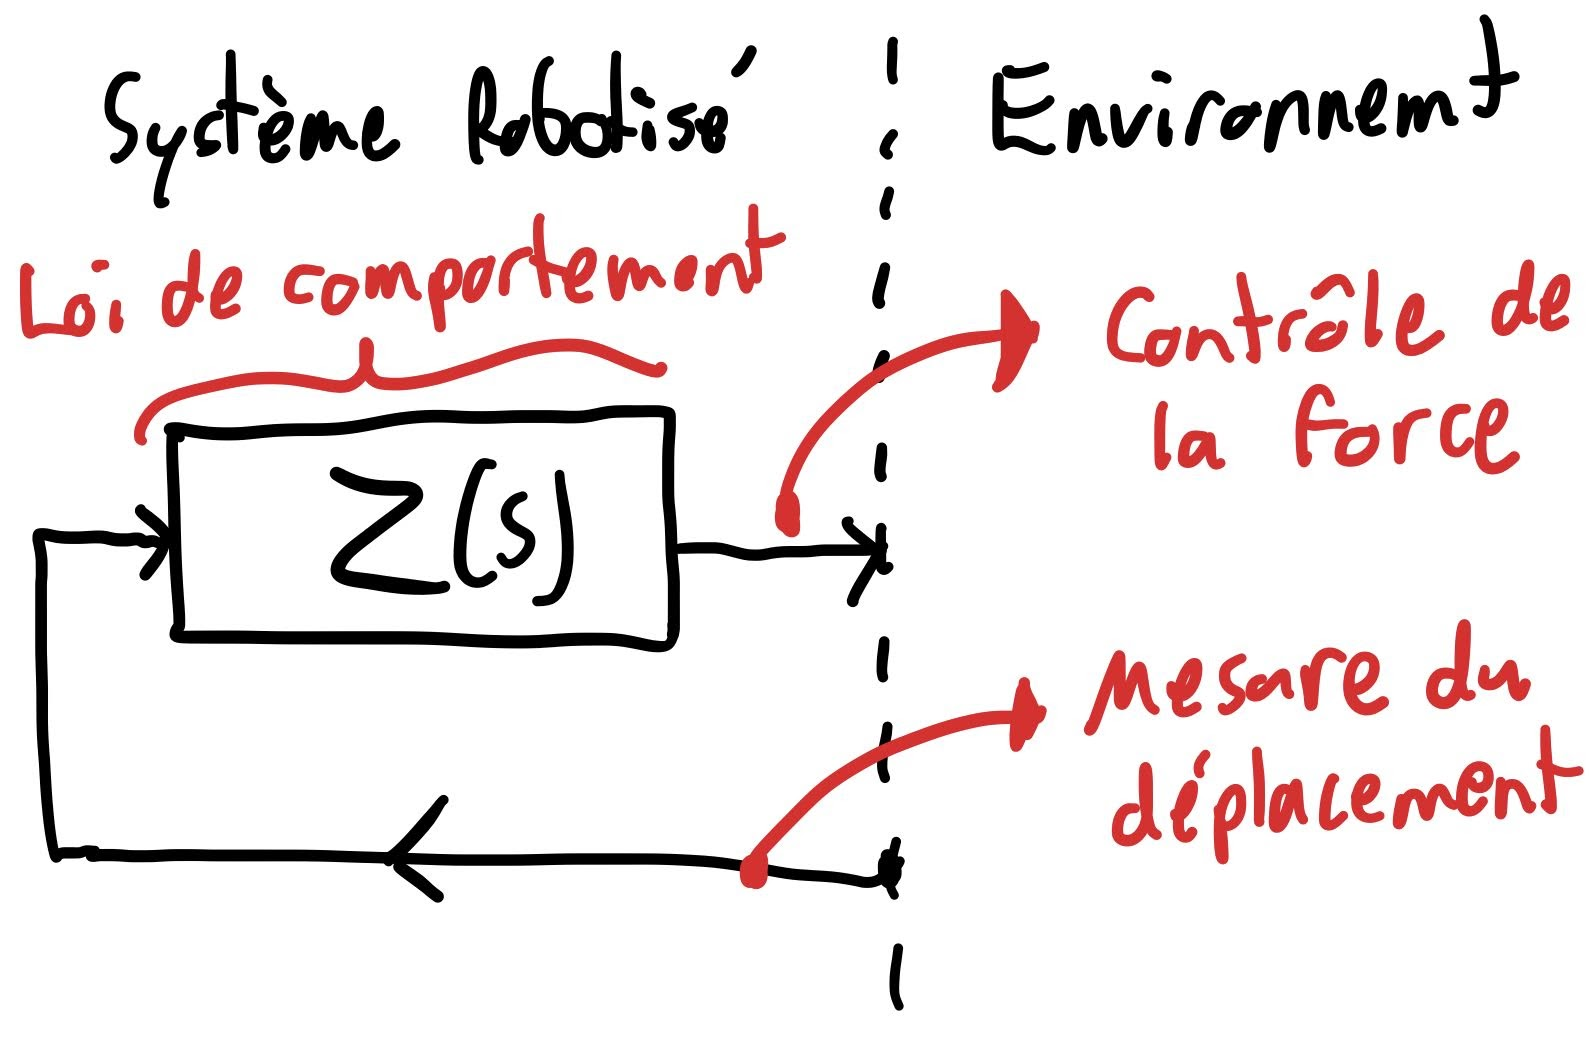
\includegraphics[width=0.40\textwidth]{fig/impedancecontrolbloc.jpg}
				\label{fig:impedancecontrolbloc}}
				%%%%
				\hspace{30pt}
				%%%%
				\subfloat[Commande en \textbf{admittance}]{
				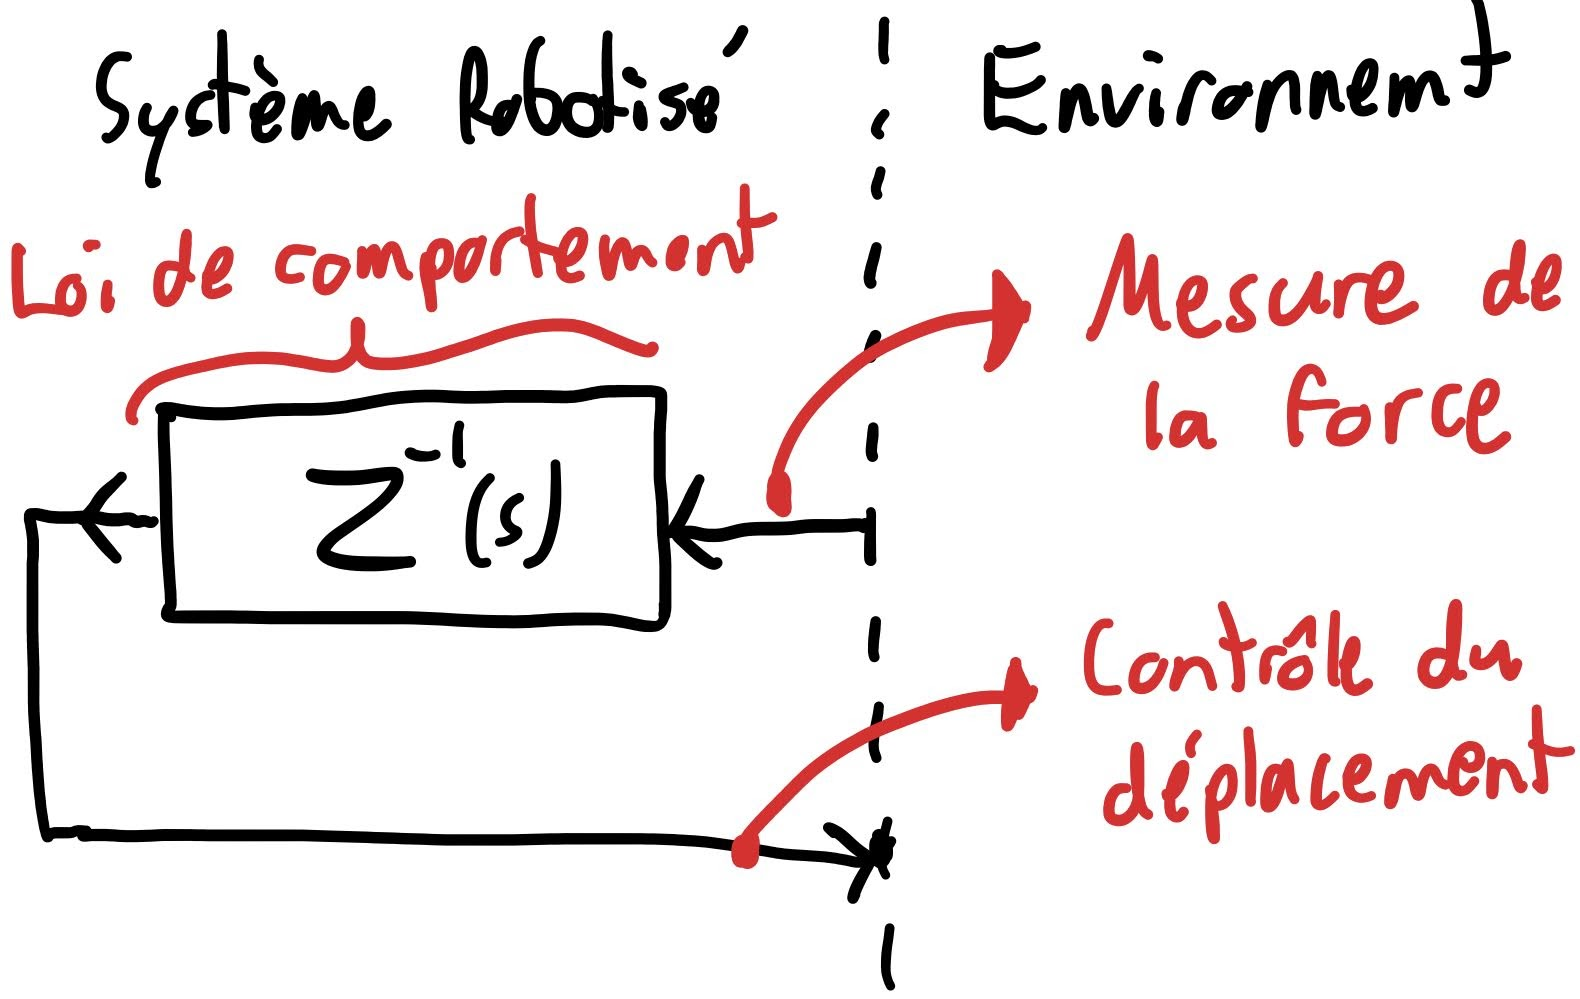
\includegraphics[width=0.40\textwidth]{fig/admitancecontrolbloc.jpg}
				\label{fig:admitancecontrolbloc}}
        \caption{Deux façon d'imposer une loi de comportement qui relie la force au déplacement.}
				\label{fig:impedanceadmitancecontrolbloc}
\end{figure}
%%%%%%%%%%%%%%%%%%%%%%%%%%%%%%%%%%%%%%%%%%%%%%%%%%%%%%%%%%%%%%%%%

\textbf{Note:} Les loi de comportement sont souvent décrit avec des fonctions de transfert dans le domaine de Laplace pour une notation compacte. La fonction $Z(s)$ est utilisée pour décrire l'impédance: le signal de force $f(s)$ divisé par le signal de déplacement $x(s)$ dans le domaine de Laplace. L'admittance $Z(s)$ est l'inverse de la fonction d'impédance. 
%%%%%%%%%%%%%%%%%%
\begin{align}
\text{Impédance:} \quad Z(s) = \frac{f(s)}{x(s)} \quad\quad \text{Admittance:} \quad Y(s) =  \frac{1}{Z(s)} = \frac{x(s)}{f(s)}
\end{align}
%%%%%%%%%%%%%%%%%
Un système mécanique avec une inertie $m$, un amortissement linéaire $b$ et une rigidité $k$ a une impédance égale à:
%%%%%%%%%%%%%%%%%%
\begin{align}
Z(s) = m s^2 + b s + k 
\end{align}
%%%%%%%%%%%%%%%%%
L'opération de multiplié le signal de déplacement par l'impédance $Z(s)$ est équivalent dans le domaine temporel à :
%%%%%%%%%%%%%%%%%%
\begin{align}
f(s) = Z(s) x(s) = \left( m s^2 + b s + k \right) x(s) \quad \Longleftrightarrow \quad 
f(t) = m \frac{d^2}{dt^2} x(t) + b \frac{d}{dt} x(t) + k x(t) 
\end{align}
%%%%%%%%%%%%%%%%%


\paragraph{Exemple} Une loi de comportement qui est souvent désirable d'implémenter est la loi de \textit{Hooke}, i.e. un ressort. Comme illustré à la Figure \ref{fig:impedanceadmitancespring}, l'approche impédance de résume à mesurer un signal de position $x$ et le multiplier par une constante de rigidité $k$ pour obtenir le force à appliquée. L'approche admittance se résume à mesurer un signal de force $f$ et le diviser par la constante de rigidité $k$ pour obtenir le déplacement $x$ à imposer. On utilise parfois la notion de compliance $C=1/k$ qui est l'inverse de la rigidité. 
%%%%%%%%%%%%%%%%%%%%%%%%%%%%%%%%%%%%%%%%%%%%%%%%%%%%%%%%%%%%%%%
\begin{figure}[H]
				%\vspace{-10pt}
        \centering
				\subfloat[Commande en \textbf{impédance}]{
				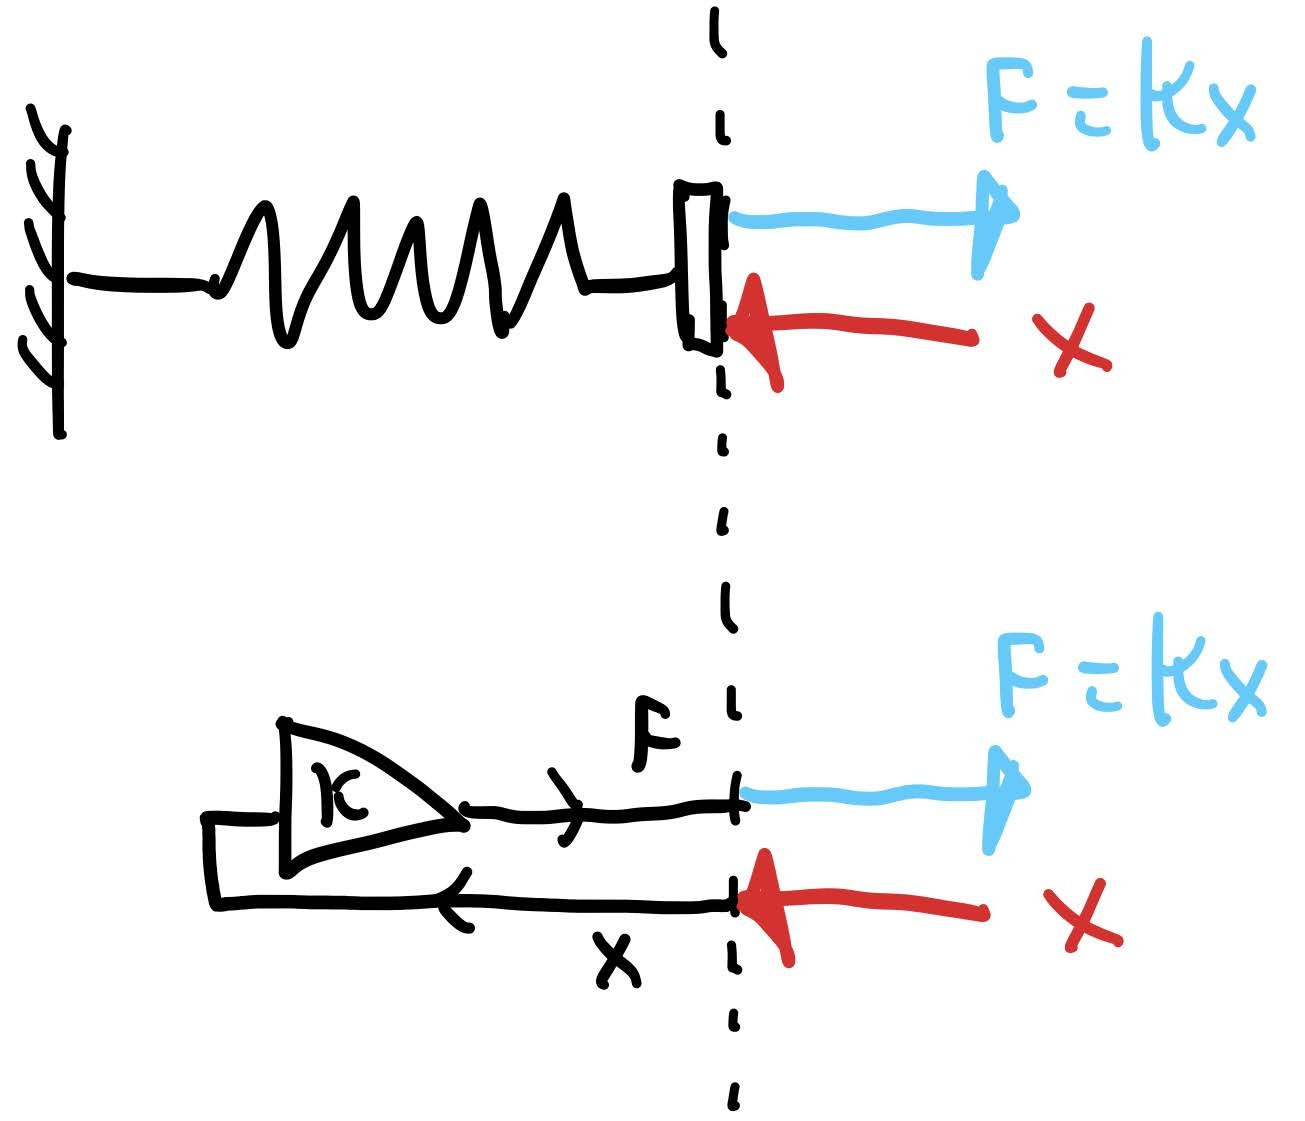
\includegraphics[width=0.40\textwidth]{fig/impedancecontrolspring.jpg}
				\label{fig:impedancecontrolspring}}
				%%%%
				\hspace{5pt}
				%%%%
				\subfloat[Commande en \textbf{admittance}]{
				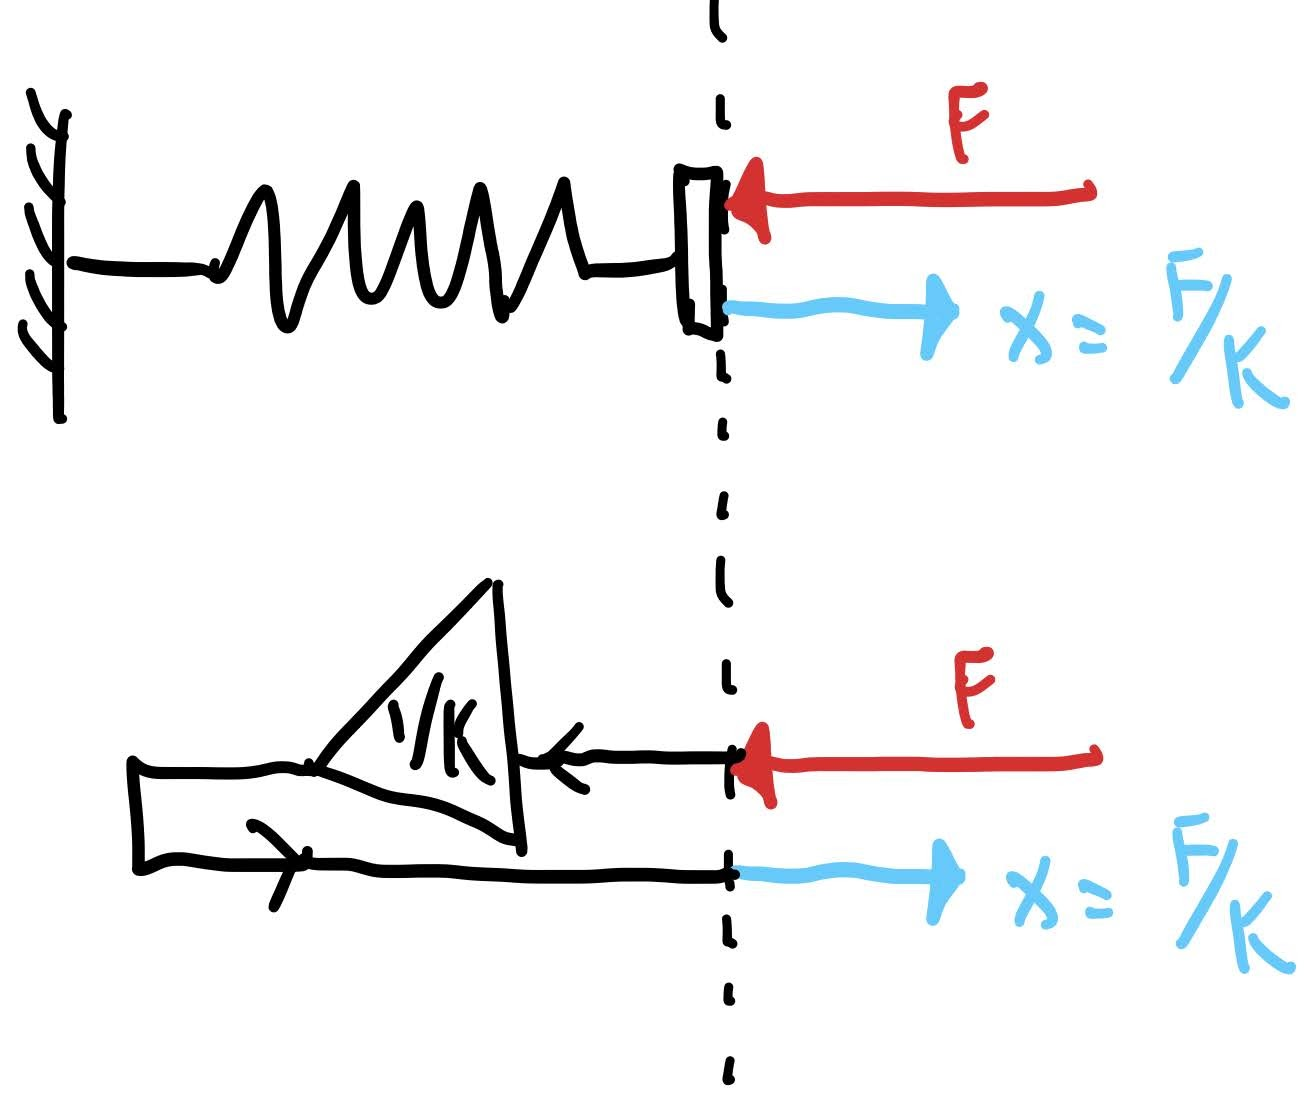
\includegraphics[width=0.40\textwidth]{fig/admitancecontrolspring.jpg}
				\label{fig:admitancecontrolspring}}
        \caption{Imposition d'une loi de comportement $f=kx$ (ressort)}
				\label{fig:impedanceadmitancespring}
\end{figure}
%%%%%%%%%%%%%%%%%%%%%%%%%%%%%%%%%%%%%%%%%%%%%%%%%%%%%%%%%%%%%%%%%

En pratique, se qui va guider le choix d'une approche ou d'une autre est principalement le type d'actionneur utilisé dans le système. L'approche par impédance est plus naturelle pour un système avec des actionneurs qui sont des sources de forces (moteur électrique sans réducteur, cylindre pneumatique, etc.), tandis que l'approche par admittance est plus naturelle pour les systèmes avec des actionneurs qui sont plus facilement contrôlable en position ou vitesse (i.e. des sources de déplacement) comme la plupart des moteurs électriques jumelés à des grandes réductions dans les robots industriels. La Figure \ref{fig:impedanceadmitancesex} illustre deux implémentations possibles pour émuler la loi de \textit{Hooke}.
%%%%%%%%%%%%%%%%%%%%%%%%%%%%%%%%%%%%%%%%%%%%%%%%%%%%%%%%%%%%%%%
\begin{figure}[H]
				%\vspace{-10pt}
        \centering
				\subfloat[Commande en \textbf{impédance}]{
				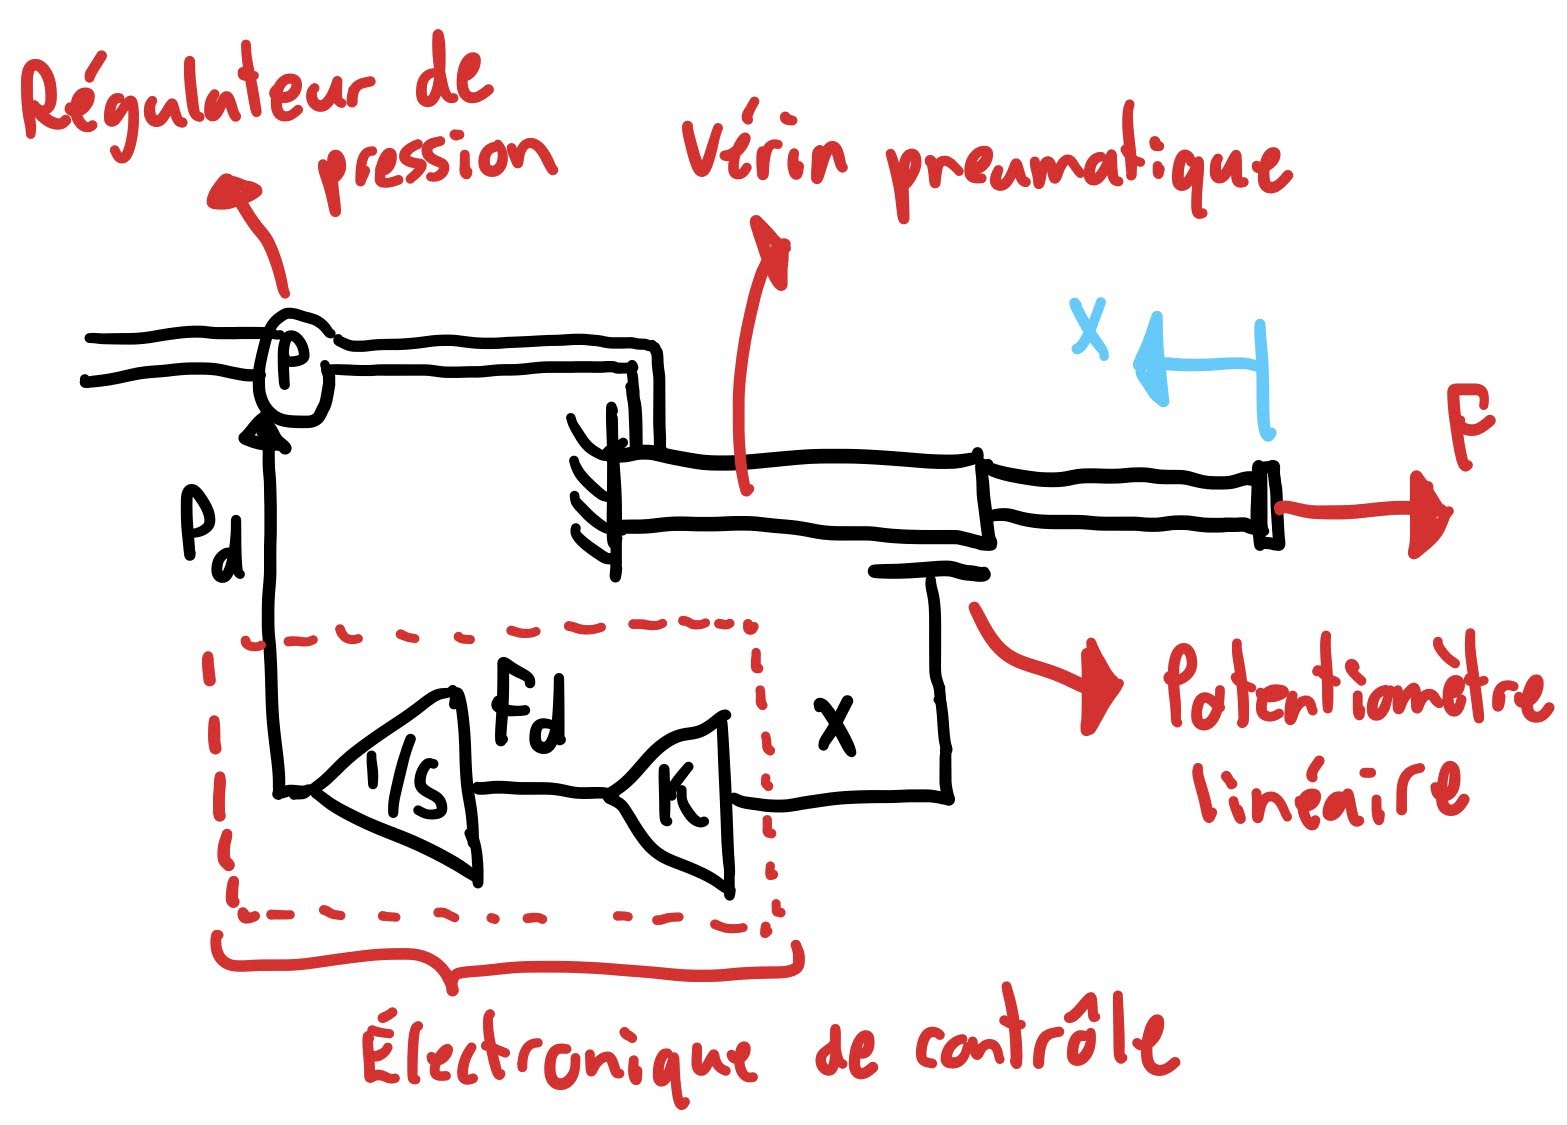
\includegraphics[width=0.45\textwidth]{fig/impedancecontrolpiston.jpg}
				\label{fig:impedancecontrolpiston}}
				%%%%
				\hspace{5pt}
				%%%%
				\subfloat[Commande en \textbf{admittance}]{
				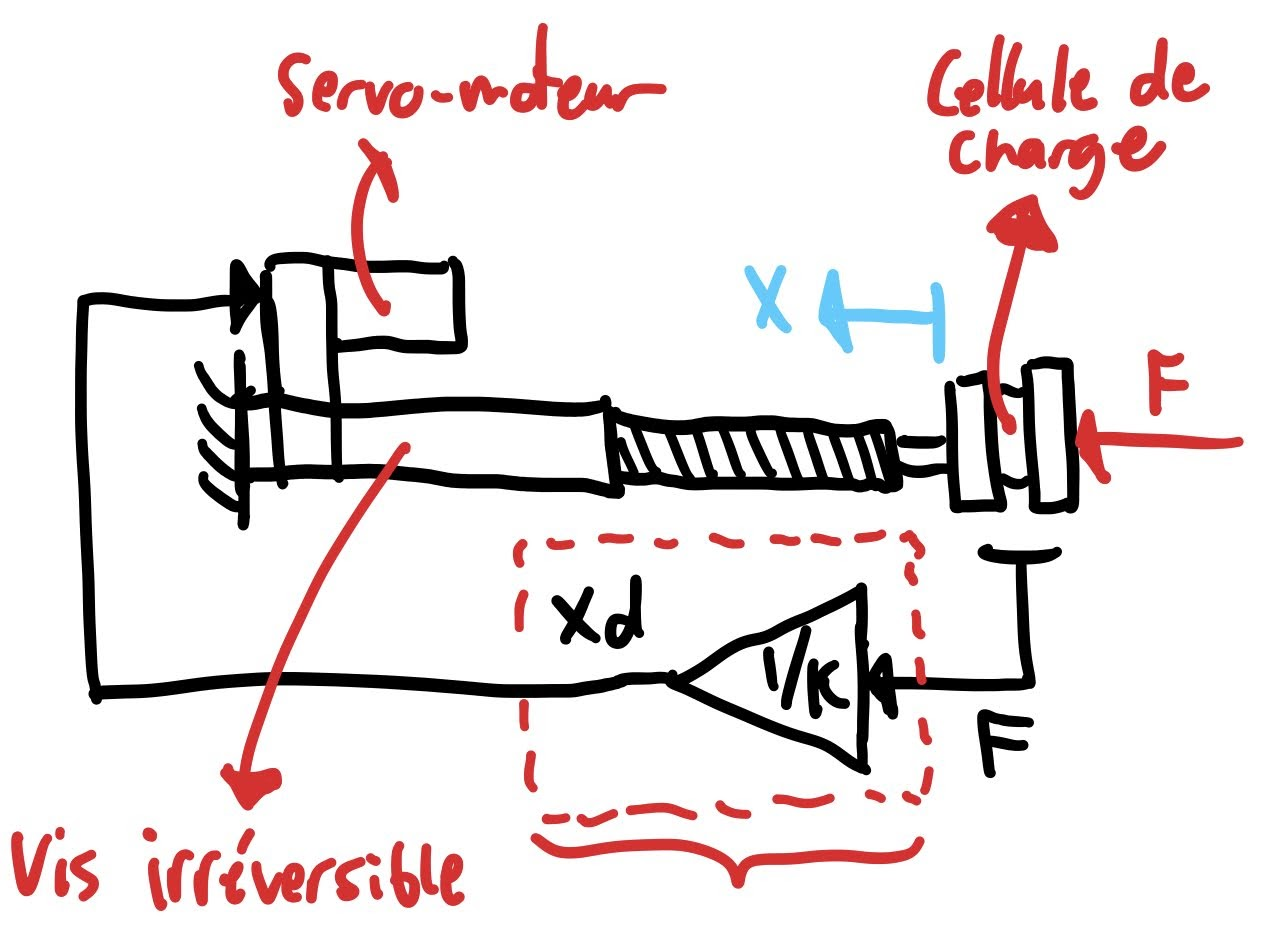
\includegraphics[width=0.45\textwidth]{fig/admitancecontrolservo.jpg}
				\label{fig:admitancecontrolservo}}
        \caption{Deux exemples d'implémentation de commande pour une loi de comportement $f=kx$ (ressort)}
				\label{fig:impedanceadmitancesex}
\end{figure}
%%%%%%%%%%%%%%%%%%%%%%%%%%%%%%%%%%%%%%%%%%%%%%%%%%%%%%%%%%%%%%%%%
Généralement, l'approche en impédance jumelée à des actionneurs à faible résistance hautement réversible (le plus proche possible d'une source de force pure) est idéale pour bien émuler des loi de comportement pour des petites impédances. La performance est toutefois limitée pour émuler des rigidités très élevée. Cette approche est généralement utilisée par les systèmes haptiques. À l'inverse, l'approche en admittance avec des actionneurs irréversible (le plus proche possible d'une source de position), est idéale pour émuler de très grandes impédances. La performance est toutefois limitée pour émuler un comportement très compliant (peu de résistance) car l'accélération et la vitesse des actionneurs sont limités en pratique. Cette approche est généralement utilisée par les robots collaboratif industriels (CoBot). 

Les sections suivantes ce concentre sur les lois de commande haut-niveau, i.e. la coordination spatiale de plusieurs joints pour obtenir des lois de comportement soit exprimées dans l'espace des joints ou de la tâche comme illustré à la Figure \ref{fig:stiffnesscontrol}. Dans ces sections il est considéré que les actionneurs sont soit des sources parfaites de force ou des sources parfaites de déplacement. La performance des boucles en forces/impédance/admittance implique une analyse de la dynamique bas-niveau des actionneurs qui est plutôt traité au chapitre \ref{sec:actuatorcontrol}. 


%%%%%%%%%%%%%%%%%%%%%%%%%%%%%%%%%%%%%%%%%%%%%%%%%%%%%%%%%%%%%%%
\begin{figure}[H]
				%\vspace{-10pt}
        \centering
				\subfloat[Dans l'espace des joints]{
				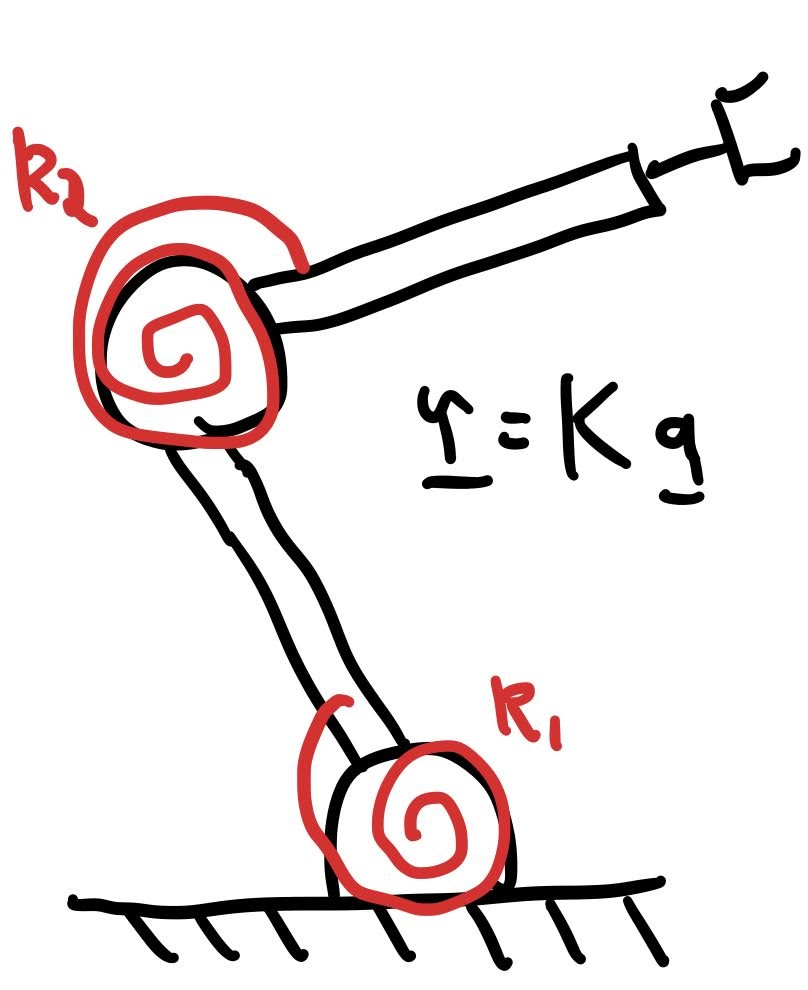
\includegraphics[width=0.40\textwidth]{fig/jointspacestiffness.jpg}
				\label{fig:jointspacestiffness}}
				%%%%
				\hspace{5pt}
				%%%%
				\subfloat[Dans l'espace de la tâche]{
				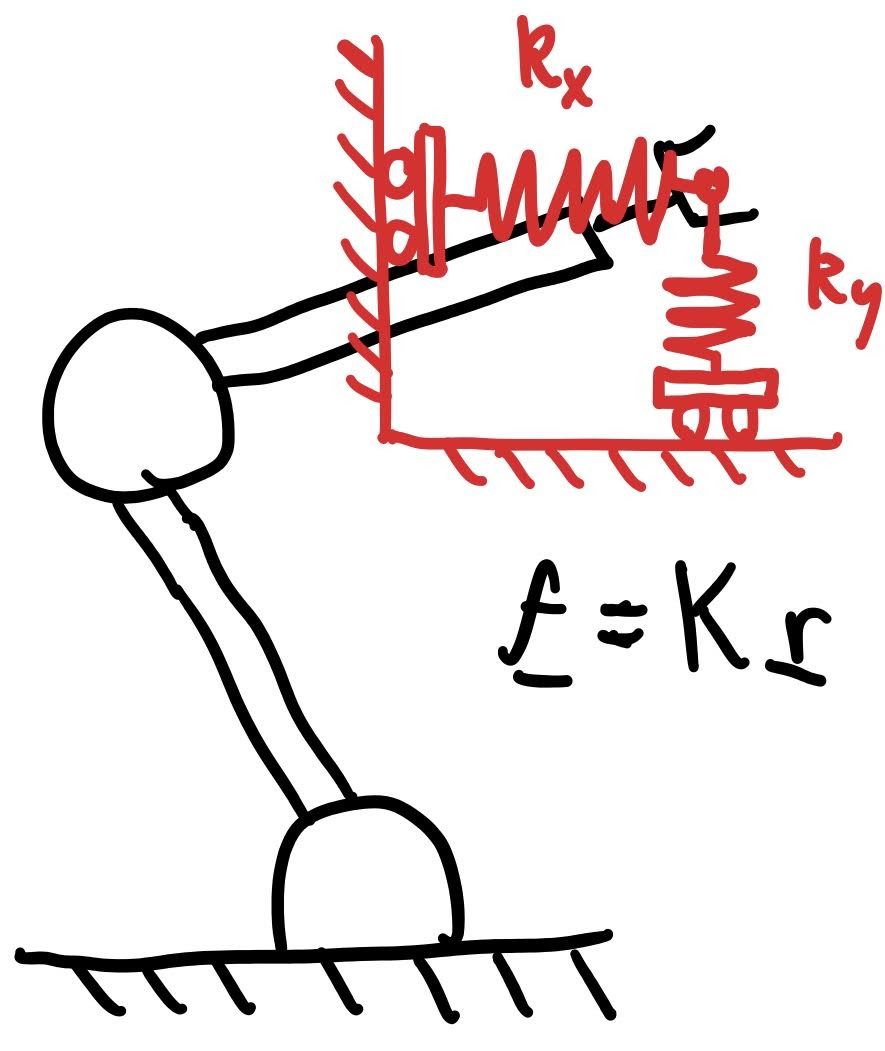
\includegraphics[width=0.40\textwidth]{fig/taskspacestiffness.jpg}
				\label{fig:taskspacestiffness}}
        \caption{Commande de la rigidité/compliance d'un robot}
			\label{fig:stiffnesscontrol}
\end{figure}
%%%%%%%%%%%%%%%%%%%%%%%%%%%%%%%%%%%%%%%%%%%%%%%%%%%%%%%%%%%%%%%%%


%%%%%%%%%%%%%%%%%%%%%%%%%%%%%%%%%%%%%%%%%%%%%%%%%%%%%%%%%%%%%%%%%
\subsection{Commande en impédance aux joints}
\label{sec:jointimpcontrol}

Pour des robots avec des actionneurs contrôlés en force ou couple, la commande en impédance aux joints se résume à relié le déplacement mesuré aux joints aux efforts à chaque joint. Dans le cas le plus simple, comme illustré à la Figure \ref{fig:jointspacestiffness}, on peut commander des couples moteurs proportionnel aux déplacement angulaire des joints, ce qui est équivalent à émuler des ressorts angulaires sur chaque joint. De façon général on pourrait émuler des ressorts-amortisseurs sur chaque joint avec la loi de commande:
%%%%%%%%%%%%%%%%%%
\begin{align}
\col{\tau} = K \col{q}_e + B \col{\dot{q}}_e
\label{eq:jointspaceimpe}
\end{align}
%%%%%%%%%%%%%%%%%
ou $\col{q}_e = \col{q}_d - \col{q}$, i.e. l'erreur par rapport à la configuration de référence ou les ressorts sont "au repos". Les matrices $K$ et $B$ sont respectivement une matrice de coefficients de rigidité et d'amortissement, et sont diagonales normalement puisque le comportement de chaque joint est indépendant. On note ici que pour le cas diagonal, la loi de commande est équivalente à plusieurs boucle d'asservissement indépendantes en position de type Proportionnel-Dérivé. 

\textbf{Compensation de friction: } Les systèmes robotiques vont normalement avoir de la dissipation naturelle présente dans les joints (roulements, engrenage, etc.). Si la friction naturelle est significative et plus grande que l'amortissement qu'on désire émuler, les coefficients de friction $B$ pourrait être négatif pour appliquer une force opposée à la friction naturelle. La matrice $B$ pourrait être définie par:
%%%%%%%%%%%%%%%%
\begin{align}
B = B_{d} - B_{sys}
\end{align}
%%%%%%%%%%%%%%%%%
ou $B_{d}$ est les coefficients d'amortissement que l'on désire émuler et $B_{sys}$ est les coefficients d'amortissement naturel du robot. Il est toutefois risqué en pratique de tenter de totalement compenser la friction dans les joints d'un robot, car si la compensation est légèrement plus forte que la friction naturelle le système se retrouve instable. 

\textbf{Note sur l'émulation de l'inertie: } On pourrait être tenté de rajouter un terme de type $M \col{\ddot{q}}_e$ à l'équation \eqref{eq:jointspaceimpe} pour rajouter l'option d'émuler un effet inertiel sur chaque joint. Toutefois il y a un problème de causalité à une telle opération. L'accélération n'est pas un état du système mais résulte de l'application de forces sur le système incluant $\col{\tau}$. Donc les couples dépendraient de l'accélération, qui dépend des couples, qui dépendraient de l'accélération, qui dépend des couples etc. En pratique, l'accélération mesurée serait celle d'un instant légèrement passé dû au temps de calcul et aux filtres dans les capteurs, et la rétroaction de la mesure de l'accélération risque de déstabiliser le système.


%%%%%%%%%%%%%%%%%%%%%%%%%%%%%%%%%%%%%%%%%%%%%%%%%%%%%%%%%%%%%%%%%
\subsection{Commande en impédance de l'effecteur}
\label{sec:effimpcontrol}

Pour la commande en impédance de l'effecteur d'un robot, c'est la relation force-déplacement de l'effecteur qu'on l'on impose au système:
%%%%%%%%%%%%%%%%%%
\begin{align}
\col{f}_e  =  K \col{r}_e + B \col{\dot{r}}_e 
\end{align}
%%%%%%%%%%%%%%%%%
que l'on peut interpréter comme un ressort-amortisseur virtuel qui relit l'effecteur du robot à sa position cible comme illustré à la Figure \ref{fig:impedanceeffector}. Le ressort-amortisseur virtuel produit une force virtuelle $\col{f}_e$ désirée à l'effecteur qui est traduite en commande de couple grâce à la relation statique d'un manipulateur:
%%%%%%%%%%%%%%%%%%
\begin{align}
\col{\tau} = J(\col{q})^T  \underbrace{ \left[ K \col{r}_e + B \col{\dot{r}}_e \right] }_{\col{f}_e}
\end{align}
%%%%%%%%%%%%%%%%%

La Figure \ref{fig:impedanceeffectorbloc} illustre cette loi de commande avec un schéma bloc. La première étape du contrôleur est de calculer la position et la vitesse de l'effecteur à partir des capteurs sur les joints. Il faut donc ici utilisé la cinématique directe et la cinématique-différentielle directe. Ensuite la position et la vitesse de l'effecteur sont comparées à la position et la vitesse désirée. L'erreur en termes de position et vitesse est convertie en force cartésienne basé sur la loi de comportement désirée (l'impédance è l'effecteur). Finalement cette force cartésienne est convertie en couple aux joints grâce au Jacobien du robot manipulateur. On peut aussi ajouter une compensation de gravité, voir la section \ref{sec:impcontrolconvergence}. 
%%%%%%%%%%%%%%%%%%%%%%%%%%%%%%%%
\begin{figure}[H]
	\centering
		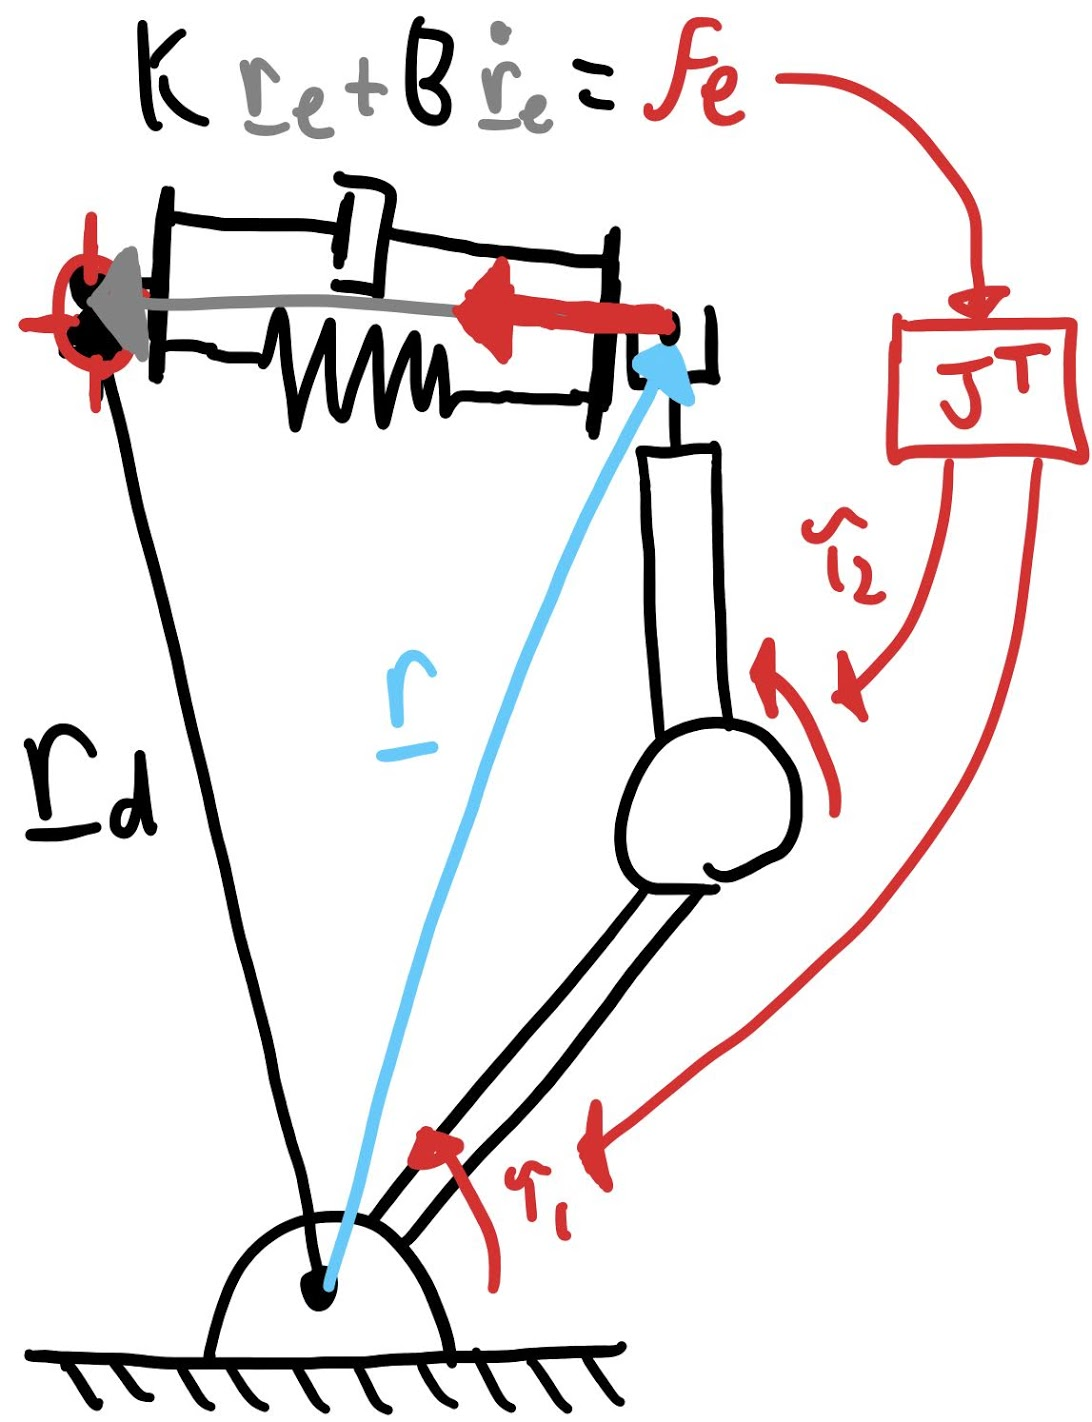
\includegraphics[width=0.4\textwidth]{fig/impedanceeffector.jpg}
	\caption{Commande de l'impédance de l'effecteur d'un robot : interprétation géométrique}
	\label{fig:impedanceeffector}
\end{figure}
%%%%%%%%%%%%%%%%%%%%%%%%%%%%%%%%


%%%%%%%%%%%%%%%%%%%%%%%%%%%%%%%%
\begin{figure}[H]
	\centering
		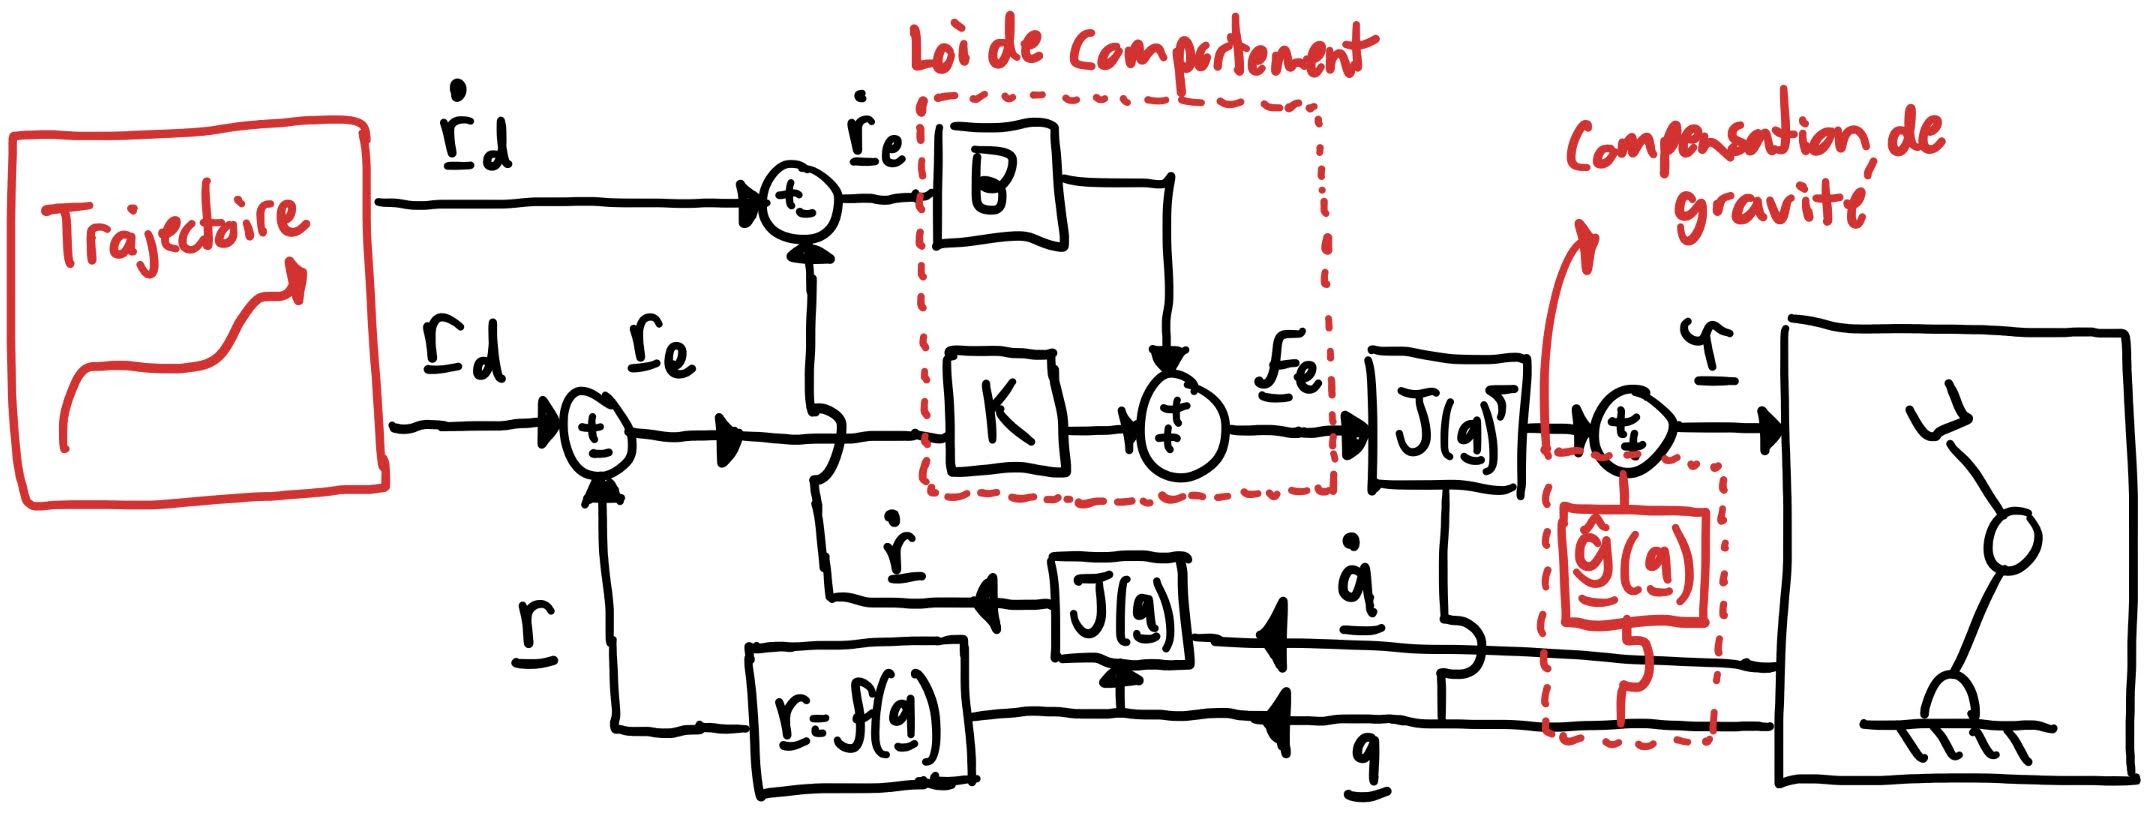
\includegraphics[width=0.99\textwidth]{fig/impedanceeffectorbloc.jpg}
	\caption{Commande de l'impédance de l'effecteur d'un robot : schéma bloc}
	\label{fig:impedanceeffectorbloc}
\end{figure}
%%%%%%%%%%%%%%%%%%%%%%%%%%%%%%%%

%%%%%%%%%%%%%%%%%%%%%%%%%%%%%%%%%%%%%%%%%%%%%%%%%%%%%%%%%%%%%%%%%%%%%%%%%%%%%%%%%
\subsection{Compensation de gravité et erreur finale des commandes en impédance}
\label{sec:impcontrolconvergence}



\subsection{Commande en admittance aux joints}
\label{sec:jointadmcontrol}

%%%%%%%%%%%%%%%%%%
\begin{align}
\dot{\col{q}} = Y(s) \col{\tau}_{c}
\end{align}
%%%%%%%%%%%%%%%%%

%%%%%%%%%%%%%%%%%%
\begin{align}
\dot{\col{q}} = Y(s) \col{\tau}_{c} = \left( M^{-1} \int + B^{-1}  + K^{-1} \frac{d}{dt}  \right) \col{\tau}_{c} \\
\col{q} = \frac{Y(s)}{s}  \col{\tau}_{c} = \left( M^{-1} \int \int + B^{-1} \int  + K^{-1}  \right) \col{\tau}_{c}
\end{align}
%%%%%%%%%%%%%%%%%

\subsection{Commande en admittance de l'effecteur}
\label{sec:effadmcontrol}

%%%%%%%%%%%%%%%%%%
\begin{align}
\dot{\col{q}} = \left\{ \begin{array}{c}
 J(\col{q})^{-1} \left( M^{-1} \int \col{f}_{c} + B^{-1} \col{f}_{c} + K^{-1} \frac{d}{dt} \col{f}_{c} \right)   \quad\quad \text{if $n=m$}
 \\ \\
 J(\col{q})^{\#} \, \left( M^{-1} \int \col{f}_{c} + B^{-1} \col{f}_{c} + K^{-1} \frac{d}{dt} \col{f}_{c} \right)  \quad\quad \text{if $n>m$}
\end{array}
\right.
\end{align}
%%%%%%%%%%%%%%%%%

